%##############################################################################
\chapter{Entwurf der Regelung}
\label{chap:Reglerentwurf}
%##############################################################################
%
Der Regelungsentwurf bzw. auch Reglersynthese genannt, beschäftigt sich nun mit der Frage wie der Regler für eine gegebene Strecke entworfen werden kann. Hierfür werden zunächst die Forderungen quantifiziert und danach geeignete Methoden ausgewählt, mit denen die Regler Parameter entsprechend ermittelt werden können. 
%
\section{Forderungen an den geschlossenen Regelkreis}
\label{sec:Forderungen}
%
Ein Regelkreis wird nach vier Gesichtspunkten ausgelegt \cite{MSF05,Lunze10}
%
\begin{itemize}
	\item Stabilität des geschlossenen Regelkreises
	\item Sollwertfolge und Störunterdrückung
	\item Dynamikanforderungen an den Regelkreis
	\item Robustheit des Regelkreises
\end{itemize}
%
Im Weiteren werden die genannten Anforderungen an den Regelkreis erläutert.
%
\subsubsection{Stabilität des geschlossenen Regelkreises}
%
Als Grundsatz gilt, dass der geschlossene Regelkreis stabil sein muss. Dies bedeutet, dass er bei einer Anregung von außen (Sollwertsprung, Störgröße) nur endliche Ausgangssignale erzeugt. Mathematisch bedeutet dies, dass die harmonischen und partikulären Lösungen der Differenzialgleichung Realteile $\Re\{\lambda_{i}\} < 0$ besitzen und somit das Einschwingverhalten stabil ist und abklingt. Für $t\rightarrow \infty$ geht das Ausgangsverhalten auf das stationäre Verhalten des Regelkreises über. Für die Analyse des geschlossenen Regelkreises existieren grundsätzlich zwei Stabilitätsbegriffe:
%
\begin{itemize}
	%
	\item \textbf{Asymptotische Stabilität:} Ein geschlossener Regelkreis wird als asymptotisch stabil bezeichnet, wenn alle Polstellen einen negativen Realteil besitzen.
	\begin{equation}
	\begin{aligned}
	\Re\{\lambda_{i}\}< 0,\,\forall \lambda_{i} \in \mathcal{N}
	\end{aligned}
	\end{equation}
	%
	\item\textbf{Eingangs/Ausgangs Stabilität:} Der geschlossene Regelkreis wird als E/A-Stabil bezeichnet, wenn das Integral der Gewichtsfunktion nicht gegen $\infty$ strebt. 
	\begin{equation}
	\begin{aligned}
	\int_{0}^{\infty}{\left|g(t)\right|}\text{d}t<\infty
	\end{aligned}
	\end{equation}
	Dies ist für Eingrößensysteme jedoch meist gleichbedeutend mit der asymptotischen Stabilität.
\end{itemize}
%
\subsubsection{Sollwertfolge und Störunterdrückung}
%
Um Sollwertfolge im geschlossenen Regelkreis zu sichern, muss der Regelkreis zunächst stabil sein. Im Weiteren wird gefordert, dass die Regelgröße $y(t)$ der Führungsgröße $w(t)$ asymptotisch folgt. Dies ist gleichbedeutend mit
%
\begin{equation*}
\begin{aligned}
%
\lim\limits_{t\rightarrow\infty}\underbrace{\left(w(t)-y(t)\right)}_{e(t)}=0.
%
\end{aligned}
\end{equation*}  
%
Für diese Forderung muss allerdings bekannt sein, für welche Art von Signalen (sprungförmig, rampenförmig, parabelförmig) der Regelkreis ausgelegt werden soll, wie bereits in Kapitel~\ref{sec:Klassifikation} angesprochen. In der Praxis ist die Auslegung auf sprungförmige Führungs- und Störsingale üblich, da sie eine breite Klasse von Signalen abdeckt. Man spricht auch davon, dass der Regelkreis keine bleibende Regelabweichung besitzt
%
\begin{equation*}
\begin{aligned}
%
e(t\rightarrow\infty)=0
%
\end{aligned}
\end{equation*}  
%
bzw. stationär genau ist. Es ist interessant zu erwähnen, das diese Eigenschaft nur von der strukturellen Auswahl des Reglers abhängt (Reglertyp), jedoch nicht von den Parametern des Reglers \cite{Lunze10}. 
%
\subsubsection{Dynamikanforderungen an den Regelkreis}
%
Die Dynamikanforderungen an den Regelkreis legen fest, wie schnell der Regelkreis den Sollwert erreichen soll oder wie er auf ein Störsignal reagieren darf. Diese Anforderungen werden oft in Bezug auf die Größe der Führungs- und Störsignale formuliert (als normierte Größen). Die Führungsprungantwort $h_{\text{W}}(t)$ des geschlossenen Regelkreises ist in Abbildung~\ref{fig:FuehrungsSprung} dargestellt.
%
\begin{figure}[h!]
	\centering
	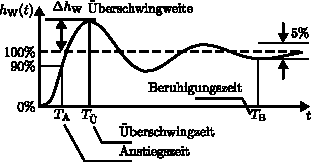
\includegraphics[width=0.68\linewidth]{Abbildungen/Systemanalyse/PDF/Sollwertfolge.pdf}
	\caption{Führungssprungantwort des geschlossenen Regelkreises \cite{Lunze10}}
	\label{fig:FuehrungsSprung}
\end{figure}
%
Es können Vorgaben für gewisse Zeitwerte der Antwort, nämlich die Anstiegszeit $T_{\text{A}}$ (90\% des stationären Endwerts) und die Überschwingzeit $T_{\text{Ü}}$ (Auftreten der höchsten Überschwingung) bestehen. In gewissen Fällen kann es sinnvoll sein, auch eine Beruhigungszeit $T_\text{B}$ festzulegen, die angibt, ab wann die Sprungantwort einen gewissen Wertbereich um den Sollwert nicht mehr verlässt. Nicht immer ist es zwingend notwendig $w(t)-y(t)=0$ zu fordern und so kann in manchen Fällen auch eine bleibende Regelabweichung zulässig sein. Jedoch wird auch gleichzeitig gefordert, dass Störgrößen ausgeregelt werden. Auch für diesen Fall gibt es Anforderungen hinsichtlich der Dynamik und des Überschwingens der Störsprungantwort $h_{\text{Z}}(t)$, siehe Abbildung~\ref{fig:StoerVerhalten}.  
%
\begin{figure}[h!]
	\centering
	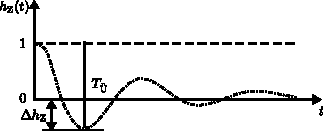
\includegraphics[width=0.68\linewidth]{Abbildungen/Systemanalyse/PDF/Stoergroessenausregelung.pdf}
	\caption{Störgrößensprungantwort des geschlossenen Regelkreises \cite{Lunze10}}
	\label{fig:StoerVerhalten}
\end{figure}
%
Der Regelkreis unterdrückt die sprungförmige Störung, welche zum Zeitpunkt $t=0$ auftritt, mit einem gewissen zeitlichen Verhalten. Dies bedeutet, dass für $t\rightarrow\infty$ die Wirkung der Störung auf den Regelkreis vollständig ausgeregelt wird.
%
\begin{python}{}{}
	\begin{itemize}
		\item \textit{Inverses Pendel mit geregelter Bewegung}
	\end{itemize}
\end{python}
%
\subsubsection{Robustheit des Regelkreises}
%
Die Robustheit eines Regelkreises beschäftigt sich mit der Frage: Wie verhält sich der Regelkreis, wenn das Modell der Strecke nicht genau genug ist? Wenn z.B. das Streckenmodell aus der Vereinfachung eines sehr komplexen Modells entstanden ist. Oder wenn sich die Parameter der Strecke mit der Zeit ändern? All diese Unsicherheiten kann man in Modellunsicherheiten oder Modellunbestimmtheiten zusammenfassen \cite{Lunze10}. Die Robustheit des Regelkreises wird in dieser Vorlesung nicht weiter berücksichtigt. Es soll nur so viel angemerkt werden, das stationär genaue Regelkreise immer ein gewisses Maß an Robustheit gegenüber Unsicherheiten besitzen, was nicht zuletzt am Rückführungsprinzip des geschlossenen Regelkreises liegt. 
%
%##############################################################################
\section{Standard Reglertypen}
%##############################################################################
%
\subsection{P-Regler}
%
Der P-Regler stellt den grundlegendsten Reglertyp dar. Er ist sehr einfach zu realisieren, hat keine verzögernde Eigenschaft, kann aber je nach Streckentyp nicht ausreichend sein, um alle Anforderungen an den Regelkreis zu erfüllen. So ist es nur mit hoher Reglerverstärkung möglich die Regeldifferenz $e_{\infty}$, bei proportional wirkenden Strecken auszuregeln.  In manchen Fällen kann eine bleibende Regeldifferenz in Kauf genommen werden, z.B. wenn ein übergeordneter Regelkreis diese Aufgabe übernimmt. Ein Beispiel hierfür ist die Drehmonentenregelung von elektrischen Maschinen. Hier sorgt eine überlagerte Drehzahlregelung für die stationäre Genauigkeit.
%
\begin{itemize}
%
\item Übertragungsfunktion
%
\begin{equation*}
\begin{aligned}
%
G_{\text{R}}(s)=K_{\text{p}}
%
\end{aligned}
\end{equation*}
%
\item Idealisierte Sprungantwort $\rightarrow$ siehe Kapitel~\ref{chap:Modellbildung}, Abbildung~\ref{fig:pglied}
%
\item Symbol bzw. Blockschaltbild
%
\begin{figure}[h]
	\centering
	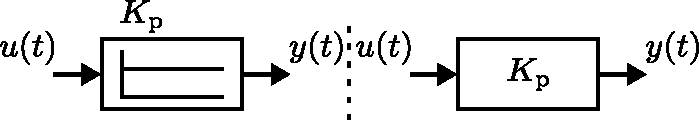
\includegraphics[width=0.65\linewidth]{Abbildungen/Modellbildung/PDF/PgliedBlock.pdf}
	\caption{Symbol, Blockschaltbild des P-Reglers}
\end{figure}
%
\end{itemize}
%
\subsection{PI-Regler}
%
Der meistgenutzte Regler in der klassischen Regelungstechnik ist der PI-Regler. Er vereint die Eigenschaften eines I-Gliedes und eins P-Gliedes und sorgt somit auch bei proportional wirkenden Strecken für stationäre Genauigkeit (vgl. Kapitel~\ref{sec:standardregelkreis}). Zudem kann durch die Nullstelle des Reglers eine Streckenzeitkonstante gekürzt werden, wodurch langsame dominante Polstelle kompensiert werden können. Dies bietet einen Freiheitsgrad für die Erfüllung der Dynamikanforderungen.
%
\begin{itemize}
	%
	\item Übertragungsfunktion
	%
	\begin{equation*}
	\begin{aligned}
	%
	G_{\text{R}}(s)&=K_{\text{P}}+\frac{K_{\text{I}}}{s}\\
	%
	G_{\text{R}}(s)&=K_{\text{P}}\left(1+\frac{1}{T_{\text{N}}s}\right),\,\, T_{\text{N}}=\frac{K_{\text{P}}}{K_{\text{I}}}
	%
	\end{aligned}
	\end{equation*}
	%
	\item Struktur des Reglers, mit der Nachstellzeit $T_{\text{N}}$ und der Verstärkung $K_{\text{P}}$. Die Nachstellzeit gibt an, wie lange der I-Anteil des Reglers benötigt, um die gleiche Stellgröße wie der P-Anteil zu erzeugen.
	%
	\begin{figure}[h]
		\centering
		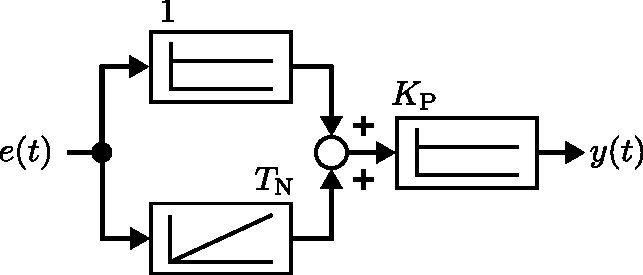
\includegraphics[width=0.5\linewidth]{Abbildungen/Reglerentwurf/PDF/PIReglerStruktur.pdf}
		\caption{Parallelstruktur des PI-Reglers}
	\end{figure}
	%
	\item Idealisierte Sprungantwort auf einen Regeldifferenzsprung $e_{0}\sigma(t)$
	%
	\begin{figure}[h]
		\centering
		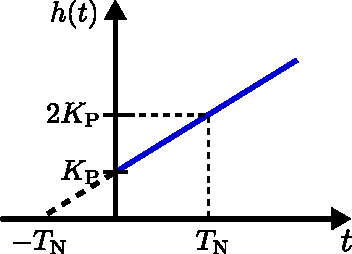
\includegraphics[width=0.375\linewidth]{Abbildungen/Reglerentwurf/PDF/PIReglerSprung.pdf}
		\caption{Sprungantwort des PI-Reglers auf einen Regeldifferenzsprung}
	\end{figure}
	%
	\item Symbol bzw. Blockschaltbild
	%
	\begin{figure}[h]
		\centering
		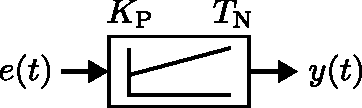
\includegraphics[width=0.3\linewidth]{Abbildungen/Reglerentwurf/PDF/PIReglerBlock.pdf}
		\caption{Blockschaltbild des PI-Reglers}
	\end{figure}
	%
\end{itemize}
%
\begin{Aufgaben}{}{}
	\begin{itemize}
		\item \textit{Stellgrößenbeschränkung (Anti-Windup) für Regler mit I-Anteil}
	\end{itemize}
\end{Aufgaben}
%
\subsection{PID-Regler}
%
Der PID-Regler wird bei schwingungsfähigen Strecken eingesetzt, da die Nullstellen auch konjugiert komplex ausgelegt werden können und somit das Stecken verhalten teilweise kompensiert werden kann (durch geschicktes kürzen der Pole). Zudem werden sie eingesetzt wenn es hohe Anforderungen an die Dynamik des Regelkreises gibt, da sämtliche langsame Pole eliminiert werden können. 
%
\begin{itemize}
	%
	\item Übertragungsfunktion
	%
	\begin{equation*}
	\begin{aligned}
	%
	G_{\text{R}}(s)&=K_{\text{P}}+\frac{\left(1+T_{\text{N}}s\right)\left(1+T_{\text{V}}s\right)}{T_{\text{N}}s}\\
	%
	G_{\text{R}}(s)&=K_{\text{P}}\left(\frac{T_{\text{N}}+T_{\text{V}}}{T_{\text{N}}}+\frac{1}{T_{\text{N}}s}+T_{\text{V}}s\right),\,\, T_{\text{V}}=\text{Vorhaltezeit}
	%
	\end{aligned}
	\end{equation*}
	%
	\item Struktur des Reglers, mit der zusätzlichen Vorhaltezeit $T_{\text{V}}$.
	%
	\begin{figure}[h]
		\centering
		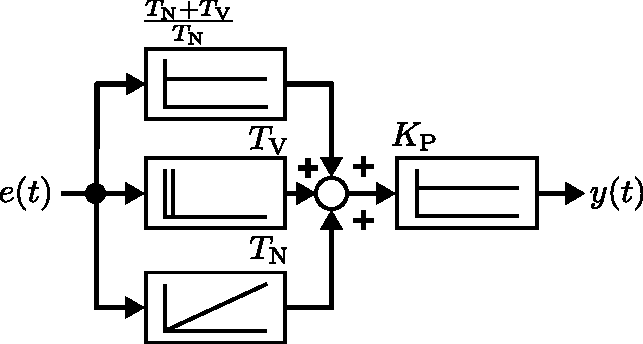
\includegraphics[width=0.55\linewidth]{Abbildungen/Reglerentwurf/PDF/PIDReglerStruktur.pdf}
		\caption{Parallelstruktur des PID-Reglers}
	\end{figure}
	%
	\item Idealisierte Sprungantwort auf einen Regeldifferenzsprung $e_{0}\sigma(t)$
	%
	\begin{figure}[h]
		\centering
		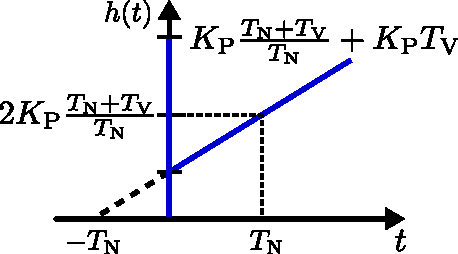
\includegraphics[width=0.45\linewidth]{Abbildungen/Reglerentwurf/PDF/PIDReglerSprung.pdf}
		\caption{Sprungantwort des PID-Reglers auf einen Regeldifferenzsprung}
	\end{figure}
	%
	\item Symbol bzw. Blockschaltbild
	%
	\begin{figure}[h]
		\centering
		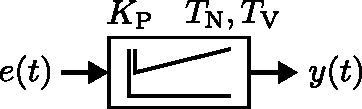
\includegraphics[width=0.3\linewidth]{Abbildungen/Reglerentwurf/PDF/PIDReglerBlock.pdf}
		\caption{Blockschaltbild des PID-Reglers}
	\end{figure}
	%
\end{itemize}
%
\newpage
%
\subsection{Technisch realisierbarer PID-Regler}
%
Das reine Differenzierglied des idealen PID-Reglers ist technisch nicht realisierbar, deshalb wird meist ein DT$_{1}$-Glied verwendet. Die Übertragungsfunktion in Parallelstruktur ergibt sich für diesen Fall zu
%
\begin{itemize}
	%
	\item Übertragungsfunktion
	%
	\begin{equation*}
	\begin{aligned}
	%
	G_{\text{R}}(s)&=K_{\text{P}}\left(\frac{T_{\text{N}}+T_{\text{V}}}{T_{\text{N}}}+\frac{1}{T_{\text{N}}s}+\frac{T_{\text{V}}s}{\left(T_{1}s+1\right)}\right),\,\, T_{\text{1}}=\text{Zeitkonstante}
	%
	\end{aligned}
	\end{equation*}
	%
	\item Struktur des Reglers, mit der zusätzlichen Zeitkonstante $T_{\text{1}}$.
	%
	\begin{figure}[h]
		\centering
		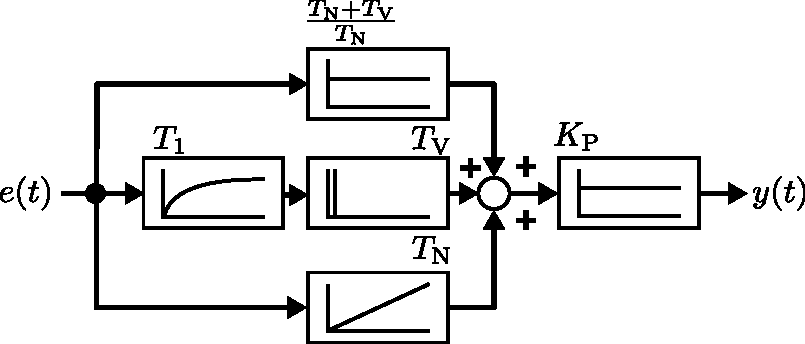
\includegraphics[width=0.6\linewidth]{Abbildungen/Reglerentwurf/PDF/PIDReglerTechStruktur.pdf}
		\caption{Parallelstruktur des PID-Reglers}
	\end{figure}
	%
	\item Idealisierte Sprungantwort auf einen Regeldifferenzsprung $e_{0}\sigma(t)$
	%
	\begin{figure}[h]
		\centering
		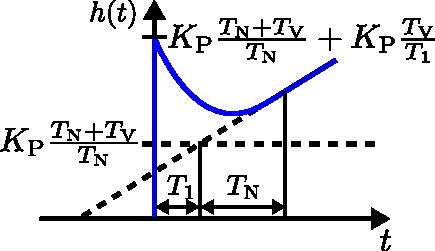
\includegraphics[width=0.4\linewidth]{Abbildungen/Reglerentwurf/PDF/PIDReglerTechSprung.pdf}
		\caption{Sprungantwort des realen PID-Reglers auf einen Regeldifferenzsprung}
	\end{figure}
	%
	\item Symbol bzw. Blockschaltbild
	%
	\begin{figure}
		\centering
		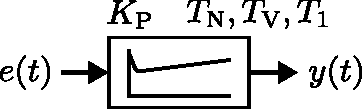
\includegraphics[width=0.3\linewidth]{Abbildungen/Reglerentwurf/PDF/PIDReglerTechBlock.pdf}
		\caption{Blockschaltbild des realen PID-Reglers}
	\end{figure}
	%
\end{itemize}
%
%##############################################################################
\section{Entwurfsverfahren für einschleifige Regelkreise}
%%##############################################################################
%
Für einschleifige Regelkreise -- Das sind Strukturen in denen es nur eine Regelgröße und eine Stellgröße gibt -- existieren eine Reihe von Entwurfsverfahren, um die Parameter des Reglers zu bestimmen, sodass der geschlossene Regelkreise vorgegebenes Verhalten nach Kapitel~\ref{sec:Forderungen} besitzt. Hierfür ist es nicht immer notwendig die Streckenparameter vollständig zu kennen, wie im weiteren Verlauf des Kapitels ersichtlich werden wird.
%
%
\subsection{Regler Entwurf mittels Einstellregeln}
%
Es existieren viele Einstellregeln für Standartregler (P-, PI-, PID-Regler), welche durch praktische Versuche an realen System entwickelt wurden. Die Beiden bekanntesten Vertreter sind jedoch das Verfahren von Ziegler-Nichols und dessen Weiterentwicklung nach Chien, Hrones und Reswick \cite{Foellinger94, MSF05, Lunze10}. Die Beiden Verfahren können auf stabile, träge Regelstrecken ohne I-Anteil und mit Totzeit angewendet werden. Im folgenden werden zwei Ausprägungen vorgestellt, wobei zunächst das Verfahren der kritischen Verstärkung gewählt wird. 
%
\subsubsection{Bestimmung der Reglerparameter bei unbekannten Strecken nach Ziegler-Nichols}
%
Die zu regelnde Strecke wird mit einem P-Regler geschlossenen und die Verstärkung $K_{\text{P}}$ des Regler so lange erhöht, bis eine Dauerschwingung auftritt, wie in Abbildung~\ref{fig:ZieglerNicholsDauer} dargestellt. Der Verstärkungswert des Reglers an diesem Punkt wird als kritische Verstärkung $K_{\text{Krit.}}$ bezeichnet.
%
\begin{figure}[h]
	\centering
	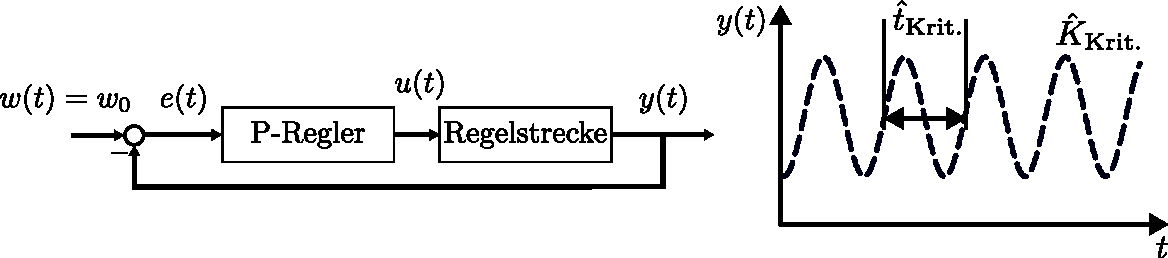
\includegraphics[width=1\linewidth]{Abbildungen/Reglerentwurf/PDF/ZieglerNicholsSchwingung.pdf}
	\caption{Dauerschwingung des geschlossenen Regelkreises an der kritischen Reglerverstärkung $K_{\text{Krit.}}$}
	\label{fig:ZieglerNicholsDauer}
\end{figure}
%
Es sei zu erwähnen, dass diese Vorgehensweise nur bei Strecken geeignet ist, die zumindest kurzfristig an der Stabilitätsgrenze betrieben werden können \cite{Lunze10}. Ist die kritische Verstärkung bestimmt, so kann über die Einstellregeln der Regler ausgelegt werden, wie in Tabelle~\ref{tab:ziegler-nichols-krit} dargestellt. Dieser Teil des Verfahrens ist für Führungsverhalten optimiert, wobei ein leicht schwingendes Verhalten der Führungssprungantwort zu erwarten ist.
%
\begin{table*}[h]\centering
	\ra{1.3}
	\caption{Einstellregeln nach Ziegler-Nichols für Streckenparameter mittels kritischer Verstärkung}
	\begin{tabular}{@{}llll@{}}\toprule
		Regler & $K_{\text{P}}$ & $T_{\text{N}}$ & $T_{\text{V}}$ \\ \bottomrule\bottomrule
		P & $0.5\,K_{\text{Krit.}}$ & - & - \\
		PI & $0.45\,K_{\text{Krit.}}$ & ${0.85}\,\hat{t}_{\text{Krit.}}$ & - \\
		PID & $0.6\,K_{\text{Krit.}}$ & ${0.5}\,\hat{t}_{\text{Krit.}}$ & ${0.12}\,\hat{t}_{\text{Krit.}}$ \\
		\bottomrule
	\end{tabular}
	\label{tab:ziegler-nichols-krit}
\end{table*}
%
\subsubsection{Entwurf bei vorheriger experimenteller Bestimmung einiger Streckenparameter}
%
In diesem Fall wird eine experimentelle Bestimmung der Streckenparametern mittels Wendetangentenverfahren (Abbildung~\ref{fig:wendetangente}) vorgenommen und danach die Parameter des Reglers aus diesen experimentell bestimmten Werten berechnet. Dabei wird vorausgesetzt, dass die Regelstrecke durch ein zeitliches Verhalten der folgenden Form approximiert werden kann:
%
\begin{equation*}
\begin{aligned}
%
G_{\text{S}}(s)&\approx \frac{K_{\text{S}}}{\left(1+T_{\text{N}}s\right)}e^{-sT_{t}}\\
%
\end{aligned}
\end{equation*}
%
Die Parameter des Wendetangentenverfahrens entsprechen $T=\hat{t}_{\text{g}}$ und $T_{t}=\hat{t}_{\text{u}}$. Es können auch andere in Kapitel~\ref{sec:experimental} vorgestellte Verfahren eingesetzt werden, um die Parameter zu bestimmen.
%
\begin{figure}[h]
	\centering
	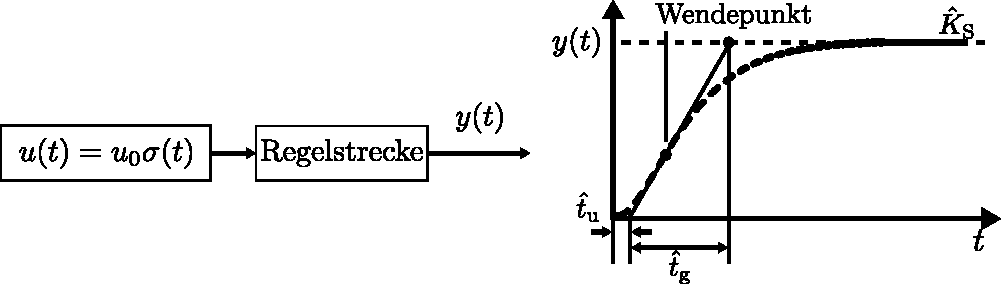
\includegraphics[width=0.9\linewidth]{Abbildungen/Reglerentwurf/PDF/ZieglerNicholsSprung.pdf}
	\caption{Sprungantwort eines PT$_{N}$-Glieds und die zu schätzenden Parameter \cite{Foellinger94}}
	\label{fig:wendetangente}
\end{figure}
%
\begin{table*}[h]\centering
	\ra{1.3}
	\caption{Einstellregeln nach Ziegler-Nichols für Streckenparameter nach Sprungantwort}
	\begin{tabular}{@{}llll@{}}\toprule
		Regler & $K_{\text{P}}$ & $T_{\text{N}}$ & $T_{\text{V}}$ \\ \bottomrule\bottomrule
		P & $\frac{\hat{t}_{\text{g}}}{\hat{K}_{\text{S}}\hat{t}_{\text{u}}}$ & - & - \\
		PI & $0.9\,\frac{\hat{t}_{\text{g}}}{\hat{K}_{\text{S}}\hat{t}_{\text{u}}}$ & ${3.3}\,\hat{t}_{\text{u}}$ & - \\
		PID & $1.2\,\frac{\hat{t}_{\text{g}}}{\hat{K}_{\text{S}}\hat{t}_{\text{u}}}$ & ${2}\,\hat{t}_{\text{u}}$ & ${0.5}\,\hat{t}_{\text{u}}$ \\
		\bottomrule
	\end{tabular}
	\label{tab:ziegler-nichols}
\end{table*}
%
Dieser Teil des Verfahrens ist für Störverhalten optimiert und besitzt eine Dämpfung $0.2<d<0.3$. Es bleibt zu erwähnen, das dieses Verfahren auch dann angewendet werden, wenn die Strecke nicht an der Stabilitätsgrenze betrieben werden darf.
%
\begin{itemize}
	\item Vorteile: 
	\begin{itemize}
		\item Sehr einfach umsetzbar.
		\item Regelstrecke muss nicht vollständig bzw. gar nicht bekannt sein.
		\item Vollständig Systematischer Entwurf.
	\end{itemize}
	\item Nachteile:
	\begin{itemize}
		\item Nur für Regelkreise geeignet die keine hohen Dynamikanforderungen haben.
		\item Die Regelstrecke muss an der Systemgrenze (Grenzstabilität) betrieben werden können, falls keine Messungen erfolgen können.
		\item Die Regelstrecke darf keinen I-Anteil enthalten. 
		\item Nur für Standardregler geeignet.
	\end{itemize}
\end{itemize}
%
\subsection{Reglerentwurf am Pol- / Nullstellendiagramm (Wurzelortskurve)}
\label{sec:WokEntwurf}
%
Beim Wurzelortskurvenverfahren wird die Lage des dominierenden Polpaars des geschlossenen Regelkreises aus den Dynamikanforderungen berechnet. Danach wird mittels verschiedener Entwurfsregeln versucht, einen Regler zu finden, mit dem diese Lage erreicht werden kann. Der Entwurf selbst erfolgt vollständig im Pol-Nullstellen Diagramm und schließt von der Lage der Pole des offenen Regelkreises und der Wurzelorte, die sich durch Variation der Reglerverstärkung ausbilden, auf das dominante Polpaar des geschlossenen Regelkreises.

Zunächst werden die Dynamikanforderungen an den geschlossenen Regelkreis quantifiziert. Hierfür wird angenommen, dass die Führungsübertragungsfunktion $G_{\text{W}}(s)=\frac{G_{0}(s)}{1+G_{0}(s)}$ durch ein PT$_{2}$-Glied approximiert werden kann.
%
\begin{equation*}
\begin{aligned}
%
G_{\text{W}}(s)&\approx \frac{1}{\left(T^{2}s^{2}+2dTs+1\right)}\\
%
&\approx \frac{\omega^{2}_{0}}{s^{2}+2d\omega_{0}s+\omega^{2}_{0}}
%
\end{aligned}
\end{equation*}
%
Für diese Übertragungsfunktion kann nun eine approximierte Führungssprungantwort der Form
%
\begin{equation*}
\begin{aligned}
%
h_{\text{W}}(t)&\approx 1-\frac{1}{\sqrt{1-d^{2}}}\cdot e^{-d\omega_{0}t}\cdot\sin\left(\left(\omega_{0}\sqrt{1-d^{2}}\right)t+\text{arccos}(d)\right)\\
%
\end{aligned}
\end{equation*}
%
abgeleitet werden. Die Parameter dieser Sprungantwort, die in Abbildung~\ref{fig:FuehrungsSprung} eingeführt wurden, lassen sich aus den folgenden Gleichungen bestimmten
%
\begin{equation*}
\begin{aligned}
%
\text{Dämpfungsgerade} &\rightarrow \cos(\varphi_{\text{d}})=d\\
\text{Überschwingweite} &\rightarrow \Delta h_{\text{W}}=e^{-\frac{\pi d}{\sqrt{1-d^{2}}}}=e^{-\pi\cot(\varphi_{\text{d}})}\\
\text{Überschwingzeit} &\rightarrow T_{\text{Ü}}=\frac{\pi}{\omega_{0}\sqrt{1-d^{2}}}=\frac{\pi}{\omega_{\text{e}}}\\
 \text{Beruhigungszeit 5 \% um den Endwert} &\rightarrow T_{5\%} \approx \frac{3}{\omega_{0}d}.
%
\end{aligned}
\end{equation*}
%
Die genannten Parameter werden nun in eine Pollage im PN-Diagramm übersetzt (siehe Abbildung~\ref{fig:WurzelEntwurf}) und ergeben einen Bereich in dem sich die Pole des geschlossenen Regelkreises befinden sollen. Hierbei sollte darauf geachtet werden, dass ein Bereich ausgewählt wird in welchem das Zeitverhalten liegen darf. Beispielsweise eine minimale und maximale Überschwingzeit bzw. Überschwingweite, denn der exakte Entwurf für ein definiertes Polpaar ist nur in Sonderfällen möglich.
%
\begin{figure}[h]
	\centering
	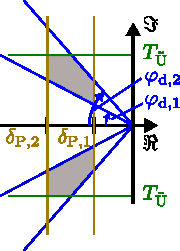
\includegraphics[width=0.3\linewidth]{Abbildungen/Reglerentwurf/PDF/PNEntwurf.pdf}
	\caption{Bestimmung der Polage des geschlossenen Regelkreises im PN-Diagramm}
	\label{fig:WurzelEntwurf}
\end{figure}
%
Danach wird der Entwurf durchgeführt. Hierfür wird ein geeigneter Regler auswählt und dessen Nullstellen und Pole so platziert, dass die gewünschte Pollage des geschlossenen Regelkreises bestmöglich erreicht werden kann. Für die Konstruktion der Wurzelortskurve nutzt man die Information aus der charakteristischen Gleichung
%
\begin{equation*}
\begin{aligned}
%
F_{0}(s)&=1+G_{\text{R}}(s)G_{\text{S}}(s)=1+G_{0}(s)\\
%
F_{0}(s)&=1+K\tilde{G}_{\text{R}}(s)G_{\text{S}}(s)=1+K\tilde{G}_{0}(s)
%
\end{aligned}
\end{equation*}
%
Welche die Lage der Pole des geschlossenen Regelkreises eindeutig beschreiben. Denn die Lösungen (Wurzelorte) der Gleichung $1+K\tilde{G}_{0}(s)=0$ ergeben die Pole des geschlossenen Regelkreises. Durch den Verstärkungsfaktor $K$, welcher dem Regler beigemessen wird, kann folglich die Lage der Pole verändert werden. Rein rechnerisch erfüllen die Wurzelorte im PN-Diagramm folgende Gleichung
%
\begin{equation*}
\begin{aligned}
%
K\frac{\prod_{i=1}^{q}\left(s-s_{\text{N},i}\right)}{\prod_{i=1}^{n}\left(s-s_{\text{P},i}\right)}=-1
%
\end{aligned}
\end{equation*}
%
Aus dieser Gleichung ergeben sich die wesentlichen Konstruktionsregeln, welche in dieser Vorlesung jedoch nicht weiter untersucht werden sollen. Vielmehr soll ein Augenmerk auf die anschauliche Erläuterung des Verlaufs der Wurzelortskurve gelegt werden. Dieser kann folgendermaßen erläutert werden:
\begin{itemize}
	%
	\item Die Wurzelorte (Pollagen des geschlossenen Regelkreises) starten für die Verstärkung $K=0$ in den Polen des offenen Regelkreises, denn
	%
	\begin{equation*}
	\begin{aligned}
	%
	0&=1+K\hat{G_{0}}(s)=1+K\frac{\hat{Z_{0}}(s)}{\hat{N_{0}}(s)}\\
	%
	&=\hat{N_{0}}(s)+K(\rightarrow 0)\hat{Z_{0}}(s)\\
	%
	&=\hat{N_{0}}(s)\\
	%
	\end{aligned}
	\end{equation*}
	%
	\item Wird die Verstärkung erhöht verschieben sich die Pole, bis sie für eine unendlich große Verstärkung $K\rightarrow\infty$ entweder in den Nullstellen des offenen Regelkreises (bei gleicher Anzahl von Polen und Nullstellen) oder im unendlichen. Meist gibt es eine geringere Anzahl Nullstellen, sodass $q$ Äste der Wurzelortskurve in Nullstellen und $n-q$ Äste im unendlichen enden.
		\begin{equation*}
	\begin{aligned}
	%
	0&=1+K\hat{G_{0}}(s)=1+K\frac{\hat{Z_{0}}(s)}{\hat{N_{0}}(s)}\\
	%
	\text{bei}\,\, n=q \quad &=\hat{N_{0}}(s)+K(\rightarrow \infty)\hat{Z_{0}}(s)\\
	%
	&=\hat{Z_{0}}(s)\\
	%
	\text{oder ohne Nullstellen} \quad &=\hat{N_{0}}(s)+K(\rightarrow \infty), \quad \text{denn} \quad \hat{Z_{0}}(s)=1\\
	%
	&=\hat{N_{0}}(s)+\infty
	%
	\end{aligned}
	\end{equation*}
\end{itemize}
%
%\begin{Aufgaben}{}{}
%	\begin{itemize}
%		\item \textit{Beispiele für Wurzelortskurven}
%	\end{itemize}
%\end{Aufgaben}
%
Für die Konstruktion der Wurzelortskurve sind zudem die Asymptoten wichtig, welche wie beim Bodediagramm den ungefähren Verlauf bestimmen lassen. Dieser ergeben sich je nach Anzahl der Pole und Nullstellen, denn jeder Polüberschuss bildet eine Asymptote aus. Im folgenden sind beispielhaft (siehe Abbildung~\ref{fig:wurzelortskurve}) Übertragungsfunktionen offener Ketten und deren zugehörige Wurzelortskurve eingezeichnet.
%
\begin{figure}
	\centering
	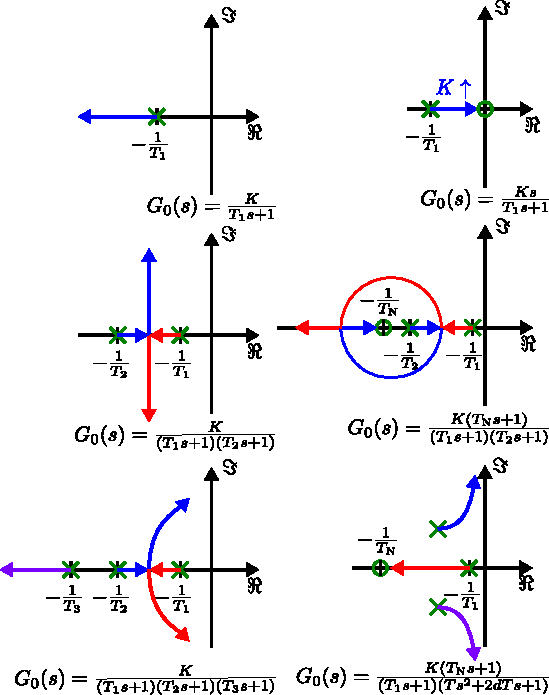
\includegraphics[width=0.8\linewidth]{Abbildungen/Reglerentwurf/PDF/Wurzelortskurven.pdf}
	\caption{Verlauf von Wurzelortskurven für verschiedene Übertragungsfunktionen $G_{0}(s)$}
	\label{fig:wurzelortskurve}
\end{figure}
%
Beim allgemeinen Entwurf geht man wie folgt vor:
%
\begin{itemize}
	\item Bestimmung der Parameter des geschlossenen Regelkreises bzw. der Führungssprungantwort aus den Dynamikanforderungen.
	\item Einzeichnen der ungefähren Pollage in das PN-Diagramm.
	\item Einzeichen der Pole der Regelstrecke $G_{\text{S}}(s)$ in das PN-Diagramm.
	\item Festlegung des Reglers, sodass die Wurzelorte für die gewünschte Pollage des geschlossenen Regelkreises über eine Veränderung der Reglerverstärkung erreicht werden können.
\end{itemize}
%
\begin{itemize}
	\item Vorteile: 
	\begin{itemize}
		\item Sehr anschaulich.
		\item Grafische Bestimmung der Wurzelorte nicht aufwendig.
		\item Computergestützte Werkzeuge für die analytische Bestimmung der Wurzelorte vorhanden.
	\end{itemize}
	\item Nachteile:
	\begin{itemize}
		\item Nur qualitative Auslegung des Regelkreises möglich.
		\item Strecken mit Totzeit lassen sich nur schwer auslegen, Totzeitglied muss approximiert werden.
		\item Kein systematischer Entwurfsweg möglich, benötigt Erfahrung.
	\end{itemize}
\end{itemize}
%
%#################################################################
\subsection{Reglerentwurf an der Frequenzkennlinie}
%#################################################################
%
Eine weitere Möglichkeit den Regelkreis zu entwerfen, bietet das Verfahren der Frequenzkennlinie. Bei diesem Verfahren wird wie bereits bei vorherigen Kapitel wiederum der geschlossene Regelkreis als ein schwingungsfähiges PT2-Glied approximiert 
%
\begin{equation*}
\begin{aligned}
%
G_{\text{W}}(s)&\approx \frac{1}{\left(T^{2}s^{2}+2dTs+1\right)}\\
%
\end{aligned}
\end{equation*}
%
Rechnet man nun von dieser Führungsübertragungsfunktion auf die Übertragungsfunktion des offenen Regelkreises zurück erhält man
%
\begin{equation}
\begin{aligned}
%
G_{0}(s)=\frac{G_{\text{W}}(s)}{1-G_{\text{W}}(s)}\approx \frac{1}{T_{\text{I}}s\left(T_{1}s+1\right)}\label{eq:offeneFrequenz}\\
%
T_{\text{I}}=2dT=\frac{2d}{\omega_{0}},\,\,\,T_{1}=\frac{T}{2d}=\frac{1}{2d\omega_{0}}.
%
\end{aligned}
\end{equation}
%
Diese Formulierung zeigt, dass der offene Regelkreis $G_{0}(s)$ für die approximierte Führungsübertragungsfunktion $G_{\text{W}}(s)$ als IT$_{1}$-Glied dargestellt werden kann. Ziel des Entwurfs ist es, für eine beliebig geartete Strecke $G_{\text{S}}(s)$ einen Regler  $G_{\text{R}}(s)$ zu finden, mit dem $G_{0}(s)$ ein IT$_{1}$-Verhalten besitzt. Werden nun noch die allgemeinen Forderungen für Sollwertfolge, Dynamik und Stabilität hinzugefügt, ergeben sich klare Regeln für die Ausgestaltung des Verlaufs der Frequenzkennlinie, wie in Abbildung~\ref{fig:FrquenzEntwurf} dargestellt.  
%
\begin{figure}[h]
	\centering
	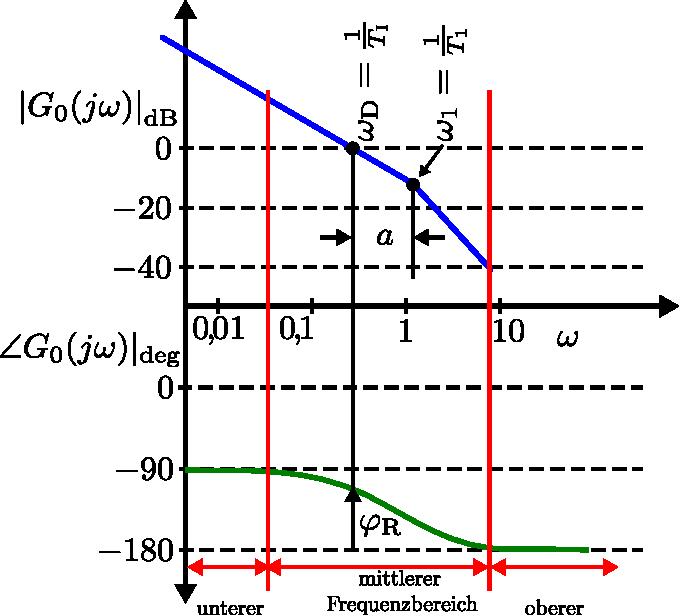
\includegraphics[width=0.6\linewidth]{Abbildungen/Reglerentwurf/PDF/Frequenzkennlinienverfahren.pdf}
	\caption{Verlauf des approximierten Frequenzgangs der offenen Kette}
	\label{fig:FrquenzEntwurf}
\end{figure}
%
Hierbei wird die Frequenzkennlinie in drei charakteristische Bereiche unterteilt:
%
\begin{description}
	%
	\item[Unterer Frequenzbereich:] In diesem Bereich soll $|G_{0}(j\omega)|_{\text{dB}}$ möglichst groß sein. Dies entspricht der Forderung, dass $G_{\text{W}}(s)\approx 1$. Denn die 1 im Nenner der Führungsübertragungsfunktion wird dann ausgeblendet. Dieser Bereich ist für das stationäre Verhalten maßgeblich. Gekennzeichnet ist dieser Bereich durch durch eine Phasenlage $\leq-90^{\circ}$, D.h. der Bereich in dem die Zeitkonstante $T_{1}$ noch keine Auswirkung auf die Phasenlage hat.
	%
	\item[Mittlerer Frequenzbereich:] In diesem Frequenzbereich soll die Durchtrittskreisfrequenz $\omega_{\text{D}}$ liegen und die zugehörige Phasenreserve $\varphi_{\text{R}}$ zumindest positiv sein. Der mittlere Frequenzbereich erstreckt sich ca. zwischen $\omega=\{0.5\omega_{\text{D}},\ldots,2\omega_{\text{D}}\}$. Im besten Fall ist die Steigung der offenen Kette in diesem Bereich nicht größer als $-20 \frac{\text{dB}}{\text{Dek.}}$. Dieser Bereich legt das dynamische Verhalten des Regelkreises fest.
	%
	\item[Oberer Frequenzbereich:] Für große Frequenzen hingegen soll die Frequenzkennlinie sowohl sehr steil verlaufen mind. $-40\frac{\text{dB}}{\text{Dek.}}$, als auch kleine Amplitudenwerte aufweisen um hochfrequente Störung bestmöglich zu unterdrücken. Somit beeinflusst dieser Bereich wesentlich das Störverhalten des geschlossenen Regelkreises. Zudem soll in diesem Bereich die Phase bereits auf $-180^{\circ}$ abgesunken sein.
\end{description}	
%
Der Abstand $a$ der beiden Zeitkonstanten hat maßgeblichen Einfluss auf die Überschwingweite $\Delta h_{\text{W}}$. Dies kann genutzt werden, um die Anzahl der Freiheitsgrade zu reduzieren und somit die Auswahl eines geeigneten Reglers zu erleichtern. Wird nun Gleichung~\ref{eq:offeneFrequenz} mit dem Parameter $a$ ergänzt ergibt sich die Darstellung
%
\begin{equation}
\begin{aligned}
%
G_{0}(s)\approx \frac{1}{aT_{1}s\left(T_{1}s+1\right)}.
%
\end{aligned}
\end{equation}
%
Diese bildet die Grundlage für das allgemeine Entwurfsverfahren. Es ergeben sich folgende Zusammenhänge für die bereits beim Wurzelortskurvenverfahren (Kapitel~\ref{sec:WokEntwurf}) eingeführten Parameter der Führungssprungantwort:
%
\begin{equation*}
\begin{aligned}
%
\text{Knickpunktabstand} &\rightarrow a = 4\frac{\left(\ln\Delta h_{\text{W}}\right)^{2}}{\pi^{2}+\left(\ln\Delta h_{\text{W}}\right)^{2}}\\
\text{Exakte Dämpfung} &\rightarrow d=\frac{\sqrt{a}}{2}\\
\text{Dämpfung am Phasenrand} &\rightarrow d\approx\frac{\varphi_{\text{d}}}{100^{\circ}}\\
\text{Überschwingzeit} &\rightarrow T_{\text{Ü}}\approx\frac{\pi}{\omega_{\text{D}}}\\
\text{Beruhigungszeit 5 \% um den Endwert} &\rightarrow T_{5\%} \approx 6T_{1}.
%
\end{aligned}
\end{equation*}
%
\begin{figure}[ht!]
	\centering
	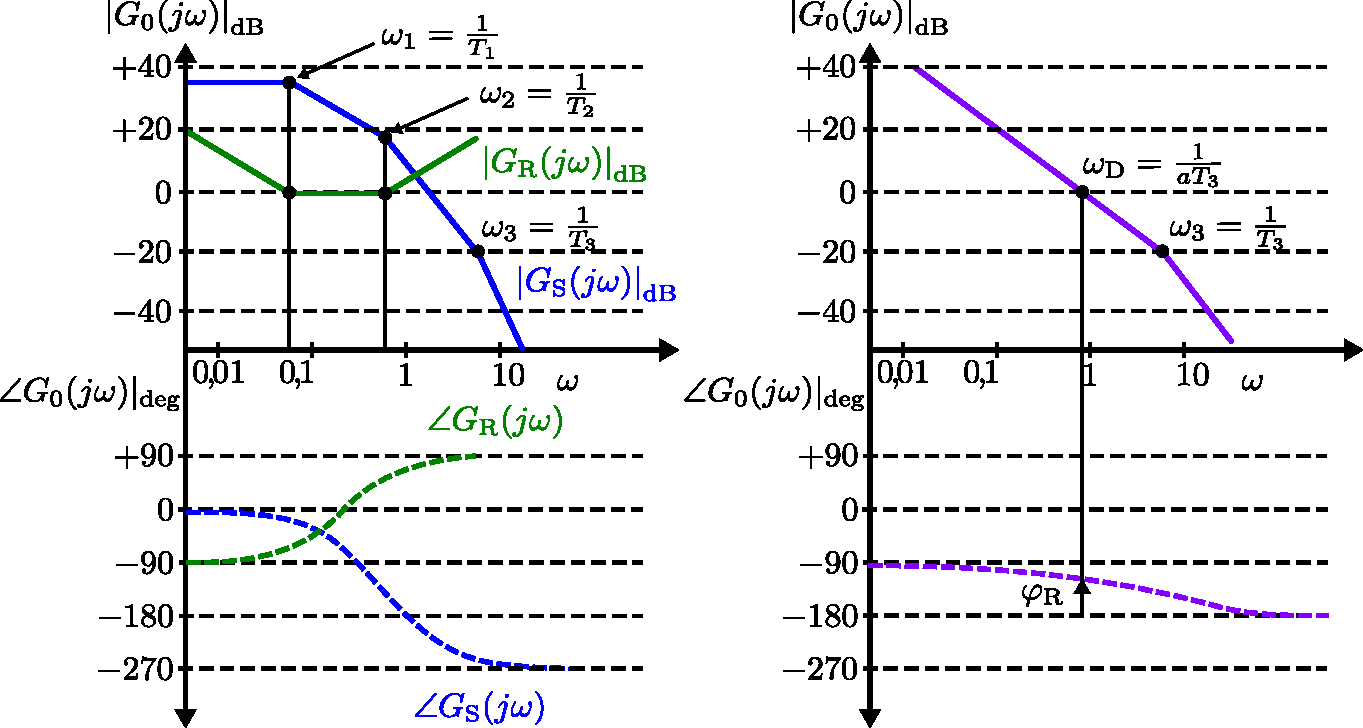
\includegraphics[width=1\linewidth]{Abbildungen/Reglerentwurf/PDF/FrequenzkennlinieEntwurf.pdf}
	\caption{Schrittweiser Entwurf eines Reglers $G_{\text{R}}(s)$ nach dem Frequenzkennlinienverfahren}
	\label{fig:frequenzkennlinie}
\end{figure}
%
%
Beim allgemeinen Entwurf geht man wie folgt vor:
%
\begin{itemize}
	\item Einzeichen der Asymptoten des Frequenzgangs der offenen Kette $G_{0}(s)$ unter der Annahme, dass der Regelkreis mit einem P-Regler $G_{\text{R}}(s)=1$ geschlossen würde. \underline{Hinweis}: Direkt die Regelstrecke $G_{\text{S}}(s)$ einzeichnen!
	\item Bestimmung der Parameter $a,\,T_{1}$ aus den Anforderungen an die Dynamik des geschlossenen Regelkreises ($\Delta h_{\text{W}},\,T_{5\%}$).
	\item Einfügen eines geeigneten Reglers, um die Frequenzkennlinie der offenen Kette in ein IT$_{1}$-Verhalten mit $T_{\text{I}},\,T_{1}$ zu überführen. Hierfür sind auch weitere Korrekturglieder erlaubt, falls die Nullstellen des Reglers nicht ausreichen, um die langsamen Pole der Strecke zu kompensieren.
	\item Bestimmung der Parameter $K_{\text{P}}$ des Reglers um die Anforderungen an die Dynamik des geschlossenen Regelkreises zu justieren ($\varphi_{\text{R}},\,T_{\text{Ü}}$).
\end{itemize}
%
%\begin{Aufgaben}{}{}
%	\begin{itemize}
%		\item \textit{Anwendungsbeispiele des Frequenzkennlinienverfahrens ohne Auslegungsparameter}
%	\end{itemize}
%\end{Aufgaben}
%
\begin{itemize}
	\item Vorteile: 
	\begin{itemize}
		\item Grafische Bestimmung mittels Bodediagramm.
		\item Totzeit kann berücksichtigt werden $\rightarrow$ Erweiterung notwendig.
		\item Kann grundsätzlich auch für offene Regelkreise ohne IT$_{1}$-Verhalten eingesetzt werden.
	\end{itemize}
	\item Nachteile:
	\begin{itemize}
		\item Nicht vollständig systematisch $\rightarrow$ nachjustieren mittels Reglerverstärkung bzw. Parameteranpassung.
		\item Unter Umständen müssen viele zusätzliche Übertragungsglieder (Regler, Korrekturglieder) eingesetzt werden.
		\item Modell der Strecke muss vollständig bekannt sein.
	\end{itemize}
\end{itemize}
%
\subsection{Reglerentwurf nach Betragsoptimum} 
%
Der Entwurf nach Betragsoptimum ist eine systematische Anwendung des Frequenzkennlinienverfahrens, welche besonders in der Antriebsregelung zum Einsatz kommt.  Der sich ergebende Regelkreis erreicht schnell den geforderten Sollwert und hat eine kurze Anstiegszeit. Zudem ist der Regelkreis gut gedämpft, wodurch nur ein sehr geringes Überschwingen der Regelgröße auftritt. Die Idee zum Entwurf basiert auf der Eliminierung der dominierenden, meist langsamen Zeitkonstante $T_{\text{A}}$ der Regelstrecke und der Vorgabe des gewünschten Verhaltens durch die weiteren Reglerparameter. Besonders geeignet ist dieses Verfahren, wenn die Regelstrecke sich in zwei Zeitkonstanten aufteilen und in folgender Form schreiben lässt.
%
\begin{equation}
\begin{aligned}
%
G_{\text{S}}(s)&\approx \frac{K_{\text{S}}}{\left(T_{\text{A}}s+1\right)\left(T_{\sum}s+1\right)}\\
%
&\text{mit}\,\,\,T_{\sum}=\sum_{k=1}^{n}T_{k}\quad \rightarrow n\,\,\,\text{kleine Streckenzeitkonstanten}\label{eq:summezeit}
%
\end{aligned}
\end{equation}
%
Durch $T_{\sum}$ werden die kleineren auftretenden Zeitkonstanten der Strecke durch ein gemeinsames P$T_{1}$-Glied approximiert. Treten Totzeiten im Streckenverhalten auf, müssen diese Ebenfalls approximiert werden, da im Entwurf keine Systematik für dies Art von Übertragungsgliedern enthalten ist. Eine gute Näherung des Totzeitgliedes lässt sich durch ein P$T_{n}$-Glied der folgenden Form erreichen.
%
\begin{equation*}
\begin{aligned}
%
G_{T_{\text{t}}}(s)&\approx \frac{1}{\left(\frac{T_{\text{t}}}{n}+1\right)^{n}}\\
%
\end{aligned}
\end{equation*}
%
Eine Approximation für $n=2$ und die Addition zur Summenzeitkonstante $T_{\sum}$ bietet bereits gute Ergebnisse.\\

Das gewünschte Verhalten des geschlossenen Regelkreises ist nun, dass der Betrag der Führungsübertragungsfunktion $|G_{\text{W}}(j\omega)|\approx1$ bis hin zu hohen Frequenzen gilt. 
Der Betrag der Führungsübertragungsfunktion ergibt sich aus Gleichung~\ref{eq:offeneFrequenz} durch die Kompensation der Streckenzeitkonstante $T_{A}$ aus Gleichung~\ref{eq:summezeit} mit einem PI-Regler ($T_{\text{N}}=T_{\text{A}}=T_{\text{I}}$). Die Zeitkonstante $T_{1}$ wiederum wird gleichgesetzt mit $T_{\sum}$. 
%
\begin{equation}
\begin{aligned}
%
|G_{\text{W}}(j\omega)|\approx \frac{K_{\text{S}}^{2}K_{\text{P}}^{2}+0\cdot\omega^{2}+0\cdot\omega^{4}}{\sqrt{T^{2}_{\text{I}}T^{2}_{1}\omega^{4}+\left(T^{2}_{\text{I}}-2T_{\text{I}}T_{\text{1}}K_{\text{S}}K_{\text{P}}\right)\omega^{2}+K_{\text{S}}^{2}K_{\text{P}}^{2}}}=1\label{eq:betragsoptimum}
%
\end{aligned}
\end{equation}
%
Aus der Forderung in Gleichung~\ref{eq:betragsoptimum} ergibt sich, dass folgende Bedingungen hierzu erfüllt werden müssen:
%
\begin{itemize}
	\item Verstärkungsfaktoren im Nenner und Zähler müssen gleich sein $K_{\text{S}}^{2}K_{\text{P}}^{2}=K_{\text{S}}^{2}K_{\text{P}}^{2}$
	\item Faktoren für den mittleren Frequenzbereich sollen gleich sein. $\left(T^{2}_{\text{I}}-2T_{\text{I}}T_{\text{1}}K_{\text{S}}K_{\text{P}}\right)\omega^{2}=0\cdot\omega^{2}$ und somit genau dann erfüllt, wenn $K_{\text{P}}=\frac{T_{\text{I}}}{2T_{1}K_{\text{S}}}$
	\item Faktoren für den oberen Frequenzbereich sollen gleich sein. $T^{2}_{\text{I}}T^{2}_{1}\omega^{4}=0\cdot\omega^{4}$ $\rightarrow$ ist nicht erfüllbar.
\end{itemize}
%
%Diese Bedingungen, welche den Betrag der Führungsübertragungsfunktion für einen weiten Frequenzbereich zu 1 setzten, sind bestmöglich erfüllt, wenn 
%%
%\begin{equation*}
%\begin{aligned}
%%
%T_{\text{I}}=2KT_{1}
%%
%\end{aligned}
%\end{equation*}
%
Setzen wir dieses Ergebnis nun in Gleichung~\ref{eq:betragsoptimum} ein, erhalten wir die sich ergebende Übertragungsfunktion des geschlossenen Regelkreises zu
%
\begin{equation}
\begin{aligned}
%
%G_{\text{W}}(s)\approx \frac{K_{\text{P}}}{T_{\text{I}}T_{1}s^{2}+T_{\text{I}}s+K_{\text{P}}}=\frac{K_{\text{P}}}{2K_{\text{P}}T^{2}_{1}s^{2}+2K_{\text{P}}T_{1}s+K_{\text{P}}}=\frac{\frac{1}{2T^{2}_{1}}}{s^{2}+\frac{1}{T_{1}}s+\frac{1}{2T_{1}}}
%
G_{\text{W}}(s)=\frac{1}{2T_{1}^{2}s^{2}+2T_{1}s+1}\approx \frac{1}{\frac{T_{I}}{K_{\text{S}}K_{\text{P}}}s+1}
%
\end{aligned}
\end{equation}
%
Vergleichen wir dieses Ergebnis mit den Parametern des PT$_{2}$-Gliedes, so erhalten wir 
%
\begin{equation}
\begin{aligned}
%
d = \frac{1}{\sqrt{2}},\, \omega_{0}=\frac{1}{\sqrt{2}T_{1}}
%
\end{aligned}
\end{equation}
%
Es ist ersichtlich, dass die Dämpfung des sich ergebenden Regelkreises mit $\frac{1}{\sqrt{2}}$ recht hoch ist, dies ist jedoch wie erwähnt ein Ziel des Entwurfsverfahrens. Im folgenden ist die qualitative Führungssprungantwort des geschlossenen Regelkreises dargestellt (siehe Abbildung~\ref{fig:betragsoptimum}). 
%
\begin{figure}[ht!]
	\centering
	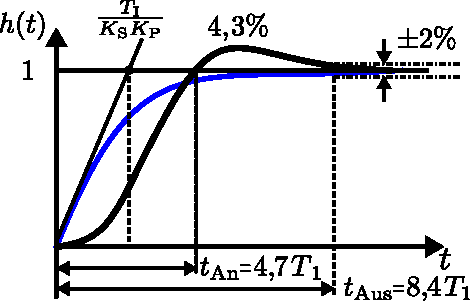
\includegraphics[width=0.45\linewidth]{Abbildungen/Reglerentwurf/PDF/SprungantwortBetragsoptimum.pdf}
	\caption{Führungssprungantwort nach Auslegung mittels Betragsoptimum (schwarze Linie) und geeignete Approximation als P$T_{1}$-Glied (blaue Linie)}
	\label{fig:betragsoptimum}
\end{figure}
%
Die Überschwingweite beträgt lediglich $4,3\%$ und nach zirka dem achtfachen der Summenzeitkonstante ist ein Sollwertsprung bereits durch die Regelgröße erreicht. Es sei noch erwähnt, dass die Summenzeitkonstante in der Regel recht klein ist.
%
%Im folgenden soll anhand der Ankerstromregelung der Gleichstrommaschine der Entwurf erläutert werden. Hierzu wird zunächst das Modell des Stromregelkreises der Gleichstrommaschine aus \cite{Stau07} ohne Herleitung eingeführt (siehe Abbildung~\ref{fig:stromregelungGSM}).
%%
%\begin{figure}[ht!]
%	\centering
%	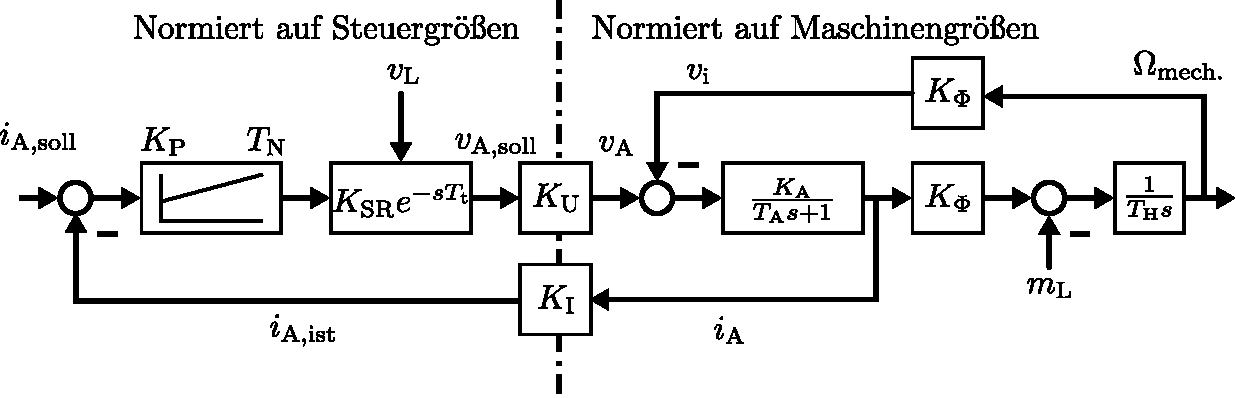
\includegraphics[width=1\linewidth]{Abbildungen/Reglerentwurf/PDF/Ankerstromregelung.pdf}
%	\caption{Normierter Ankerstromregelkreis der permanenterregten Gleichstrommaschine}
%	\label{fig:stromregelungGSM}
%\end{figure}
%%
%Wird die Rückführung zum Regler aufgetrennt und die Übertragungsfunktionen der einzelnen Blöcke zusammengefasst ergibt sich folgende Übertragungsfunktion der Strecke
%%
%\begin{equation}
%\begin{aligned}
%%
%|G_{\text{W}}(j\omega)|\approx \frac{K^{2}}{T^{2}_{\text{I}}T^{2}_{1}\omega^{4}+\left(T^{2}_{\text{I}}-2T_{\text{I}}T_{\text{1}}K\right)\omega^{2}+K^{2}}\label{eq:gsmStrecke}
%%
%\end{aligned}
%\end{equation}
%%
%%
%\subsection{Entwurf nach Symmetrischen-Optimum}
%%
%\begin{itemize}
%	\item Einführung
%	\item Auslegung (Formel)
%	\item Bedeutung im Bode Diagramm $\rightarrow$ Zeichnung
%	\item Vorfilter
%	\item Tabelle mit Auslegungsparametern für verschiedene Streckentypen
%	\item Sprungantwort $\rightarrow$ Zeichnung
%\end{itemize}
%